There are several control systems of note in an optical trapping setup. The subcarrier servo controls the accousto-optic modulators (AOMs) which take light from the carrier and frequency shift it to create the subcarrier. The trap cavity control servo and digital system are responsible for locking the cavity and reading out the cavity transfer function.

\begin{figure}[htbp]%
\centering
\includegraphics[width=.8\textwidth]{figures/photothermal/layout3}%
\caption[Simplified optical spring layout]{There are two main control loops in an optical spring system. The first is the subcarrier servo, (green box, lower right) which detunes the subcarrier a set frequency from the carrier. The second controls the laser frequency and the trap cavity input coupler to lock the cavity.}%
\label{fig:controlLoopsSimple}%
\end{figure}

\section{Subcarrier Servo}
The goal of the subcarrier servo is to red detune the subcarrier beam a set frequency away from the carrier beam. 
The required frequency shift is roughly twice the cavity pole frequency. 
With the parameters of our experiment, our cavity pole frequency was about 140 kHz, and thus our required detuning was about 300 kHz. 
There are no easily available AOMs that work in that frequency range. 
Previous experiments \cite{Corbitt07} have overcome this by shifting an entire FSR plus the desired detuning, but the FSR of our cavity is about 2 GHz, which is above the range of standard AOMs. 

Thus we chose a difference frequency scheme with two AOMs frequency shifting in opposite directions to achieve small offset (~200kHz) within a single FSR.
This system is controlled by the subcarrier servo, which is designed to lock a VCO (voltage controlled oscillator) a set frequency away from a crystal oscillator. The is accomplished through two mixers and some feedback, as shown in figure \ref{fig:subcarrierservo}.

We use directional couplers to get low-power signals from both the 80 MHz crystal oscillator and the VCO so that the majority of the power is driving the AOMs, maximizing the optical power going into the first order mode. 
The signal from the oscillator is mixed with the output of the VCO to produce a signal where the frequency is the difference between the two signals. 
This signal is then mixed with the desired offset frequency, set on the function generator, to give a low frequency error signal.
The error signal is passed through some filters in the servo, then fed into the VCO frequency modulation input.

\begin{figure}[htbp]%
\centering
\includegraphics[width=1.2\textwidth,angle=90]{figures/controls/SubcarrierServo}%
\caption[Subcarrier Servo]{Subcarrier Servo diagram. The servo locks the VCO output to the 80 MHz oscillator output, offset by the function generator. The VCO and 80 MHz output signals are taken from the directional couplers (ZMDC-10-1), which output a majority of the power through the ``Out'' terminal to the AOMs. Those signals are fed through a mixer (ZMY-3), then the output is mixed again (ZAD-8) with the function generator (200 kHz).
The function generator can be tuned from roughly 50 kHz to 2 MHz.}%
\label{fig:subcarrierservo}%
\end{figure}

We typically monitor two spots in this system: The output of the fast mixer (ZMY-3) and the drive signal from the function generator (200 kHz on the diagram). When locked, the two should have the same frequency and be phase locked. The unity gain frequency of the locked system is about 2 kHz. below that, the servo should suppress frequency noise in the AOM drive (though it will not help for sensing noise). 

%\lab\lab2013\Subcarrier_servo\20130424_freq_noise

%\section{Introduction}
%
%We're going to take a single oscillator, and beat it against a time delayed version of itself to figure out the phase noise.  This method should work for any oscillator, though there are `dead spots' in the spectrum due to resonance that we have to be careful about.
%
%Let's cover some variables...
%
%\begin{itemize}
%\item Oscillator Frequency $f_{osc} = 80 \mbox{MHz}$
%\item Speed of light in BNC cables $s = 0.66 c$
%\item Volt of mixer DC offset per radian of phase: $g_{rad}=0.34 \mbox{V/rad}$
%\item Delay Cycles $n=3$ 
%\item Time delay $T=\frac{n}{f_{osc}}$
%\item Phase noise measurement frequency $f_{meas}=1 \mbox{kHz}$  
%\end{itemize}
%
%$$A e^{i(\omega t+\phi(t))}   \otimes B e^{i(\omega (t-T)+\phi(t-T))} = A(\omega) e^{i(\omega T+\phi(t)-\phi(t-T))} $$
%
%Our friendly spectrum analyzer does an FFT on it...
%
%$$\phi(\omega) (1-e^{i\omega T}) \approx \phi(\omega) i \omega T$$
%
%then we can ask ourselves, ``how accurately can I measure this noise?''  Assuming a spectrum analyzer noise floor of $1 \mbox{nV}/\sqrt{\mbox{Hz}}$
%
%$$\phi_{min}=\frac{1 \mbox{nV}}{\sqrt{\mbox{Hz}}} \frac{1}{g_{rad}}\frac{1}{2\pi f_{meas}T}$$
%$$=\frac{1 \mbox{nRad}}{0.34\sqrt{\mbox{Hz}}}\frac{f_{osc}}{2\pi (1\mbox{kHz})(n)}$$
%$$=\frac{1 \mbox{nRad}}{0.34\sqrt{\mbox{Hz}}}\frac{f_{osc}}{2\pi (1\mbox{kHz})(n)}$$
%$$=\frac{37}{n} \frac{\mu Rad}{\sqrt{\mbox{Hz}}}$$
%
%This is the smallest phase noise that we could measure for a given $n$.  Note that, with a wavelength of about 2.5 m, it is feasable to consider an $n$ up to perhaps 20.
%
%Next question is: how does phase noise affect our noise in the cavity (in $m/\sqrt{\mbox{Hz}}$)?
%
%$$ f_n(\omega)=\frac{1}{2\pi}\frac{d}{dt}\phi_n(\omega) = \frac{\omega}{2\pi} \phi_n$$
%
%$$FSR+f_n=c/(2L+x_n)\approx\frac{c}{2L}\left(1-\frac{x_n}{2L}\right)$$
%
%current nosie estimate is $10^{-17}m/\sqrt{\mbox{Hz}}$
%
%$$f_n = \frac{c}{2L}\left(1-\frac{x_n}{2L}\right)-FSR = 1.3\times 10^{-7}$$
%
%$$\Delta x \approx \frac{\lambda_0^2}{2L}$$ distance between peaks in an FSR
%
%so our lower bound in phase noise measurement should be below
%
%$$\phi_n = f_n \frac{2\pi}{\omega}= 8.4\times10^{-10} rad/\sqrt{\mbox{Hz}}$$

\subsection{Measuring frequency noise}

We are going to look at the spectrum of the oscillators near 80 MHz to figure out the amount of frequency noise from these oscillators.  We're mostly concerned with the frequency noise in the 1 kHz band around the peak.

We begin by assuming that all voltage noise is phase noise (no change in the amplitude).  This method gives an upper limit to the noise in the system.

In the following discussion, $\omega_m$ is a measurement frequency and $\omega_c$ is the carrier frequency.

We expect the voltage output to be $V(t) = V_0 e^{i(\omega_c t + \phi(t))}$, where $\phi(t)$ is the noise in the system.

In the frequency domain,

\begin{equation}
\delta V(\omega_m) = V_0 \delta \phi(\omega_m) = \frac{2\pi V_0}{\omega_m} \delta f(\omega_m).
\label{eq:VofOmega}
\end{equation}

It is important to note that we need to sum the effects of the noise at the carrier plus 1 kHz and the carrier minus 1 kHz to get the total frequency noise.

\begin{equation}
\delta f(\omega_m)= \frac{\omega_m \delta V(\omega_m)}{2 \pi V_0}.
\label{eq:deltafSCS}
\end{equation}


We can now calculate the effect of this frequency noise on our optical trap cavity length $\delta x$.  $f_L$ is the laser frequency.

\begin{equation}
\delta x = \frac{L}{f_L} \delta f = 2.66\times10^{-16} \delta f.
\label{eq:deltax}
\end{equation}

%The noise budget gives a noise floor of $10^{-17}$, so to get in under that, we need $\delta f <<\frac{1}{26.6}$.


\subsection{Results}

With the subcarrier servo locked at approximately 200 kHz, the noises we measure are:

80 MHz Oscillator: frequency noise $5.4\times 10^{-3} \frac{\mbox{Hz}}{\sqrt{\mbox{Hz}}}$.  Position noise $1.4\times 10^{-18} \frac{\mbox{m}}{\sqrt{\mbox{Hz}}}$.

VCO: frequency noise $6.7\times 10^{-2} \frac{\mbox{Hz}}{\sqrt{\mbox{Hz}}}$.  Position noise $1.7\times 10^{-17} \frac{\mbox{m}}{\sqrt{\mbox{Hz}}}$.

Both of these values are below the expectation of laser frequency noise at 1 kHz (about $2\times 10^{-15} \frac{\mbox{m}}{\sqrt{\mbox{Hz}}}$) , so that should be acceptable.

%These noise values are OK for the 80 MHz oscillator, but not so much for the VCO.  We suspect that the 200 kHz oscillator may be the culprit.


\begin{figure}[htp]
	\centering
		\includegraphics[width=\textwidth]{figures/controls/80.png}
	\caption[80 MHz oscillator spectrum]{Spectrum of the 80 MHz crystal oscillator around 80 MHz.}
	\label{fig:80}
\end{figure}

\begin{figure}[htp]
	\centering
		\includegraphics[width=\textwidth]{figures/controls/VCO.png}
	\caption[VCO spectrum]{Spectrum of the locked VCO. The sidebands are likely caused by the function generator.}
	\label{fig:VCO}
\end{figure}



\section{Cavity control loops}

\begin{figure}[htp]
\includegraphics[width=475pt,angle=270]{figures/controls/traplockSimple.png}%
\caption{Analog parts of the locking loop. We lock the cavity (OS) using the PDH signal from the reflected RF photodiode (Refl RF). The feedback signal goes to the laser PZT for fast feedback and to the digital system for slow feedback to the OSEMs. We measure the open loop transfer function of the system by driving the ``In'' port, then measuring ``OutA'' divided by ``OutB''.}
\label{fig:traplock}%
\end{figure}

\begin{figure}[htp]
\includegraphics[width=\columnwidth]{figures/controls/traplockdig.png}%
\caption[Digital loops]{Digital parts of the locking loop. These parts are responsible for the slow feedback to the OSEM coils. The yaw and optical lever inputs are not relevant to the longitudinal trap.}%
\label{fig:traplockdig}%
\end{figure}


Here's a picture of the longitudinal trap as it stands.  In general terms, we have a cavity with position and laser feedback, which also has optical spring behavior.  Analog and digital loops are shown in figures \ref{fig:traplock} and \ref{fig:traplockdig}.

%You may notice that this layout drawing has an alphabet soup of sections and subsections. 
%I will now describe in excruciating detail what each of these things are and why we care.  


Each component has a letter associated with it, which represents the transfer function of the associated element. Each of the following sections describes an element and how it is calculated.
I am leaving out the input whitening on the analog side and the dewhitening on digital side.  They should cancel out every time, so we just leave them off.

Our goal is to be able to reconstruct the entire optical trap from the control point to the error signal.  In our measurements, we are using the injection input and the two test outputs of the Trap Servo board. Test out A serves as our error signal (OUT) and Test out B serves as our control signal (IN).  The injection happens between the two test outputs. The resulting open loop transfer function is plotted in figure \ref{fig:OLG}.
This is based on James Lough's  \cite{LoughThesis} model of the loop, which I have updated and repackaged.

%\begin{equation}
%\frac{F}{1-SO}\left[HLM+\frac{AECP+TCP}{1-PCED}\right]
%\label{eq:loop}
%\end{equation}

\begin{equation}
\frac{Out A}{Out B}=\left[FHLM+\frac{FAECP+FTCP}{1+PCED}\right]\frac{1}{1+SO}.
\label{eq:loop}
\end{equation}

There are several different parts to this equation, so we will take a moment to look at each term.  Every term in the numerator includes $F$, the Trap Servo. $FHLM$ is a loop involving the PZT drive of the laser.  $FAECP$ and $FTCP$ both rely on pushing the large mass around using the OSEM drive, but $FAECP$ does the drive through the digital system while $FTCP$ uses an analog connection. $PCED$ is the open loop transfer function of the active suspension damping for the large mass; note that this only affects the loops that are driving the large mass. $SO$ is the open loop transfer function of the optical spring acting on the small mirror, which is dependent on the separation between the two mirrors, rather than the absolute position of either.



%-360 is a product of two closed loops and one open loop.  The two closed loops are the optical spring, $(1-SO)^{-1}$, and the active seismic damping from the digital system to the OSEMs, $(1-PCED)^{-1}$.  The open loop is the sum of three paths: the feedback of the trap servo through the laser ($FHLM$), the feedback of the trap servo through the digital system to the OSEMs ($FAECP$), and the feedback of the trap servo directly to the OSEM drive ($FTCP$) 

\begin{figure}[htbp]
\centering
\includegraphics[width=\columnwidth]{figures/controls/blocks.png}%
\caption[Block diagram of the system]{Block diagram of the open loop transfer function for trap locking and operation. Two closed loops (OS and DECP) are highlighted in blue and red, respectively.}%
\label{fig:blocks}%
\end{figure}


%I'm using for reference Jim's code, TrapLoop.m, which is a Matlab class.  The code can be found in /lab/jim/newtrap. There is an example of the code in use, fitplots.m, in /lab/lab2014/TrapServo/20140423/



\subsection{A : Digital PDH feedback}

At the moment, this path has been disconnected because it was not required.  Thus we can set $A=0$.

%The input to this is the signal coming out of the Trap servo. The output is a drive signal which gets added into the OSEM drive of trap 1.  This box has a digital and an analog component.  In the analog section, the signal gets an attenuation $a = 95\Omega/2795\Omega$ via a votage divider.  After that, the signal enters the digital system, where we have the filters in the POS\_PDH\_FEEDBACK filter bank.  At the moment, the only active filter is a lowpass with a single pole at $10 \mbox{Hz}$. The -0.5 is related to the digital system input, the 40/3 is a gain set in the digital system, and the -7 is a fitting parameter.
%
%\begin{equation}
%A = a\frac{-10}{1+\imath f/(10 \mbox{Hz})}\frac{40\cdot (-0.5)\cdot-7}{3\cdot}\left[\frac{\mu\mbox{N}}{\mbox{mV}}\right]\cdot \frac{1000(\mbox{mV/V})}{10^6(\mu\mbox{N}/\mbox{N})}
%\label{eq:A}
%\end{equation}

\subsection{C : OSEM coils}

The OSEM coils convert voltage from the DAC into force on the large mirror via the OSEMs.  We have a factor of 4 in the numerator because there are 4 OSEMs acting on the mass.  The constant ($4.91793\times 10^{4}$ V/N) comes from a measurement made in October 2013 and recorded in the SUGWG logbook (entry number 439).

\begin{equation}
C = \frac{4}{4.91793\times 10^{4}\mbox{ V/N}}.                               
\label{eq:C}
\end{equation}


\subsection{D1 and D2 : Digital feedback based on optic motion}
The input to each of these blocks the is motion of a single optic relative to the OSEMs. The OSEMs put out a current proportional to the position of the mass, which is digitized.  The output is a drive signal which gets added into the OSEM drive of trap 1 and trap 2, respectively.  The position measurements from each optic have filters applied from the TRAP1\_SUSPOS and TRAP2\_SUSPOS filter banks. In D1, we have an AC coupling filter(Z: 0, P: 0.5), a highpass (Z: 1, P: 100), and a fourth order Chebychev lowpass filter at $200\mbox{Hz}$ with $1\mbox{dB}$ of passband ripple (P: $67.3977\pm\imath81.4946$, $27.9074\pm\imath196.677$ G: -0.891251).  There is also a gain of 10, which includes the filter gain, the conversion of position of the optics relative to the OSEMs into voltage, and the conversion from volts to meters in the digital system. See fig. \ref{fig:D}. 

From the Matlab code:

\begin{verbatim}
    tf = (1i*freq - 0) .* (1i*freq - 1)...
        ./ (1 + 1i*freq / 0.5)...
        ./ (1 + 1i*freq / 100)...
        ./ (1 + 1i*freq / (67.3977+1i*81.4946))...
        ./ (1 + 1i*freq / (67.3977-1i*81.4946))...
        ./ (1 + 1i*freq / (27.9074+1i*196.677))...
        ./ (1 + 1i*freq / (27.9074-1i*196.677))...
        .* -0.891251...
        .* Dgain;
\end{verbatim}


We do not consider the effects of D2 because we are not putting any active drive through it. Thus it will not shape the loop as drastically as D1. The coupling between the mirror position and the ring position drops off drastically ($f^{-2}$) above the position resonance of the glass suspension ($\approx 18\mbox{ Hz}$). As we improve the lock, we expect that we will be able to reduce or even remove active feedback on the ring.

\begin{figure}[htbp]
\includegraphics[width=\columnwidth]{figures/controls/D.png}%
\caption[D1 transfer function]{D1, the transfer function from the position of optic 1, the input coupler, to a digital drive force. }%
\label{fig:D}%
\end{figure}

\subsection{E : Force to volts}

The digital system converts the force output of digital filters into volts so that it can be sent out of the digital system to the OSEMs. We include a factor of 4 because we have 4 OSEMs.  Note that $CE = 1$.


\begin{equation}
E = \frac{1}{4} 4.91793\times 10^{4}\mbox{V/N}.
\label{eq:E}
\end{equation}

\subsection{F : Trap PDH servo}

This is the transfer function of the Trap Servo, the RF photodiode, and the mixer.  Input to this is the cavity length, read out through the PDH method. The output is a voltage. The variable `mxrpd,' which is the conversion from cavity length to the voltage output of the mixer, is dependent on power, cavity mode matching, and the PDH readout at the mixer. mxrpd, measured at full power, just below the oscillation point, is about $10^9$ V/m. See fig. \ref{fig:F}.  At the moment, we are only using the 100 Hz integrator. This has been modeled completely with the `Analog' library developed by Stefan Ballmer, rather than calculating the algebraic expressions. 

%in /software/matlab/analog.


\begin{figure}[htb]
\includegraphics[width=\columnwidth]{figures/controls/F.png}%
\caption[Calculated trap servo TF]{Calculated trap servo TF. The main components are a 1 kHz lowpass filter and a user-adjustable gain.}%
\label{fig:F}%
\end{figure}

\subsection{P : Pendulum}

The pendulum transfer function of the large mass converts a force to a displacement in the position direction.  The resonant frequency is $f_L = 1.4 \mbox{Hz}$ and the Q factor is about 200. The mass of the input coupler is $m_L = 300$ g.

\begin{equation}
%P = \frac{1}{m_L (2 \pi f_L)^2} \frac{1}{\left(1 - \left[\frac{f}{f_L}\right]^2\right)}
P = \frac{1}{4 \pi^2\left[m_L (f_L^2-f^2)+\frac{iff_L}{2Q}\right]}.
\label{eq:P}
\end{equation}

\begin{figure}[htb]
\includegraphics[width=\columnwidth]{figures/controls/P.png}%
\caption{Damped large mass pendulum transfer function.}%
\label{fig:DPloop}%
\end{figure}

\subsection{S : Suspension spring}

The glass suspension connects the small optic to the ring; it acts as a high-Q spring. An optical lever is used to damp oscillation modes other than the position mode. It converts a force to a displacement in the position direction.  The resonant frequency of the suspension is $f_s = 18 \mbox{ Hz}$ and the small mass is $m_s = 0.41 \mbox{ g}$.

\begin{equation}
S = \frac{1}{m_s (2 \pi f_s)^2}\frac{1}{\left(1 - \left[\frac{f}{f_s}\right]^2\right)}.
\label{eq:S}
\end{equation}

\subsection{O : Optical spring}

The optical spring has a transfer function that looks very much like that of a physical spring. Depending on detunings and power ratio, we should see stable or unstable behavior. One such transfer function is plotted in figure \ref{fig:O}.  We should note that optical losses before the cavity have to be considered when determining the power in the cavity, as well as the cavity detuning and angular displacements of the mirrors.  At the moment we are calculating this using Finesse \footnote{gwoptics.org/finesse/}.

\begin{figure}%
\includegraphics[width=\columnwidth]{figures/controls/O.png}%
\caption[Optical spring]{Plot of the closed loop behavior of the optical spring and the glass suspension.  
%The 1 Hz position resonance will be suppressed by the digital system damping loop}
%\caption{Optical Srping.  Single model has a single spring with power of 38 mW and a detuning of 33 kHz.  Dual model has two beams, a carrier with 295 mW detuned 355 kHz, and a subcarrier with 41 mW power detuned 260 Hz.  }%
}
\label{fig:O}%
\end{figure}

Combining this spring constant with S in a closed loop gives us the behavior of the optical spring on the small mass, and thus cavity length.  Below, in equation \ref{eq:OS_CL}, is the effect of the optical and mechanical springs on changes in the cavity length.

%\begin{figure}%
%\includegraphics[width=\columnwidth]{figures/controls/blocks2.png}%
%\caption[Block diagram of the cavity with sources of actuation]{Block diagram of the cavity with sources of actuation. Because the optical spring loop is independent of other factors, we can multiply the closed loop gain of the optical spring ($CLG$) by the electronic, mechanical and digital parts of the feedback loop.}%
%\label{fig:cavityloopblocks}%
%\end{figure}

\begin{equation}
\frac{1}{1+OS} = \frac{k_m-m\omega^2}{k_m+k_{os}-m\omega^2}.
\label{eq:OS_CL}
\end{equation}

\subsection{L : Laser PZT}

The laser PZT converts a voltage to a shift in the laser frequency. The number is taken from the product spec sheet.

\begin{equation}
L = -1.7\times 10^6 \mbox{ Hz/V}.
\label{eq:L}
\end{equation}

\subsection{M : Cavity response}

Changes in the laser frequency can be converted into an effective change in the cavity length.  The cavity length $l$ is 0.07 m. This only works for $l\gg\lambda_0$.

\begin{equation}
M=\frac{l\lambda_0}{c}.
\label{eq:loopM}
\end{equation}


\subsection{H : HV amplifier}

H is the HV amplifier (with HV bypass) which drives the laser PZT (See fig. \ref{fig:H}). 
The HV bypass was introduced to bypass the HV amplifier above its unity gain frequency to increase the feedback bandwidth.  
It is described in the SUGWG ALog in entry 412.  
The overall behavior of the amplifier and the bypass is designed to look like this simplified model:
%https://sugwg-alog.phy.syr.edu/aLOG/index.php?callRep=412 data and model in lab2013/FSS/20130908

\begin{equation}
H = \frac{70}{1+\imath f/146}.
\label{eq:Hmodel}
\end{equation}
We actually interpolate the data for this block, so that we don't run into trouble in the discrepancy region.


\begin{figure}[htbp]
\includegraphics[width=\columnwidth]{figures/controls/H.png}%
\caption{HV amplifier transfer function. Includes a high-frequency bypass to increase feedback bandwidth.}%
\label{fig:H}%
\end{figure}


\subsection{T : Analog PDH feedback to coil drivers}

This is a SR560 that operates between the Trap Servo control signal and the analog drive for the large optic OSEMs.

It is currently set to a 1 kHz 6 dB lowpass with a gain of 200, so it is modeled as 

\begin{equation}
T = \frac{200}{1 - \imath \frac{f}{1\mbox{ kHz}}}.
\label{eq:T}
\end{equation}						



\section{Photothermal effect on loops}
The photothermal effect is directly related to how close the cavity is to resonance. This is affected by the total cavity length and the frequency of the light entering the cavity. In figure \ref{fig:photothermal_blocks}, we see that the photothermal effect (Pt) can be treated as a closed loop acting on the cavity length $L_{cav}$.

\begin{figure}[htp]
\begin{center}
\includegraphics[width=.9\textwidth]{figures/controls/photothermal_blocks}
\end{center}
\caption[Loop diagram for a single degree of freedom]{%
\label{fig:photothermal_blocks}
Loop diagram for a single degree of freedom, including photothermal feedback, Pt. The optical spring loop on the left side ($k_O$, $k_m$, and $m_2$) is affected by the photothermal effect ($Pt$). We measure the behavior of the optical spring by measuring the open loop transfer function of the system at F, then dividing out the transfer functions of the control system ($HLM$, $T$, $D$, etc.). This leaves us with the closed loop transfer function of the optical spring with the photothermal effect. }
\end{figure}


\begin{figure}[htbp]
\centering
\includegraphics[width=343pt]{figures/controls/OLG.png}%
\caption{Open loop TF of the system with several different carrier detunings. Changing the carrier detuning changes the resonant frequency of the springs and their stability. Included are both measurements and corresponding models.}%
\label{fig:OLG}%
\end{figure}